\documentclass[12pt,a4paper]{article}
\usepackage[utf8]{inputenc}
\usepackage{graphicx}
\usepackage{booktabs}
\usepackage{amsmath}
\usepackage{hyperref}
\usepackage{geometry}
\usepackage{float}

\geometry{margin=1in}

\title{%
  \textbf{P15: Sentiment Classification of Texts}\\
  \vspace{0.5em}
  \large CS485 -- Project Report
}
\author{%
  Zervos Spiridon Chrisovalantis (csd4878) \\
  Drakakis Rafail (csd5310)
}
\date{\today}

\begin{document}

\maketitle
\thispagestyle{empty}

\begin{abstract}
  We implement and compare three classes of sentiment‐classification pipelines on the IMDb Movie Reviews dataset:
  \begin{enumerate}
    \item \emph{Classical ML} using TF–IDF (Term Frequency–Inverse Document Frequency) and Logistic Regression, Naive Bayes, Linear SVM
    \item \emph{Deep Learning} using PyTorch LSTM and 1D‐CNN with learned embeddings
  \end{enumerate}
  We evaluate each on accuracy, precision/recall/F1 (for classical), and inference or epoch time.  
\end{abstract}

\newpage
\tableofcontents
\newpage

\section{Introduction}
Sentiment analysis classifies text as positive or negative. We use the standard IMDb review benchmark to compare:
\begin{itemize}
  \item \textbf{Classical ML}: TF–IDF $\to$ Logistic Regression / Naive Bayes / SVM
  \item \textbf{Deep Learning}: LSTM \& 1D‐CNN over a learned embedding layer
\end{itemize}

\section{Dataset}
\begin{itemize}
  \item \textbf{Name:} IMDb Movie Reviews  
  \item \textbf{Size:} 50000 total (25000 train, 25000 test)  
  \item \textbf{Labels:} Positive (1) / Negative (0)  
  \item \textbf{Source:} \url{https://ai.stanford.edu/~amaas/data/sentiment/}
\end{itemize}

\section{Implementation Details}
\subsection{Preprocessing \& Vocabulary}
\begin{itemize}
  \item NLTK downloads guarded for \texttt{punkt}, \texttt{punkt\_tab}, \texttt{stopwords}.
  \item Lowercasing, tokenization (\texttt{word\_tokenize}), alpha‐filter, stopword removal.
  \item For deep models: build vocab from training tokens (min\_freq=2, max\_size=20000), pad/truncate to length 200.
\end{itemize}

\subsection{Feature Extraction}
\begin{itemize}
  \item \textbf{Classical:} TF–IDF (unigrams, max\_features=5000).
  \item \textbf{Deep:} learned \texttt{nn.Embedding} (dim=100).
\end{itemize}

\subsection{Models \& Hyperparams}
\begin{description}
  \item[LogisticRegression] $C=1.0$, $\ell_2$, max\_iter=1000.
  \item[MultinomialNB] $\alpha=1.0$.
  \item[LinearSVC] $C=1.0$.
  \item[LSTM] embed\_dim=100, hidden\_dim=128, single layer, trained 5 epochs, Adam lr=1e-3.
  \item[CNN] embed\_dim=100, 3 conv‐filters (sizes 3,4,5) each 100 channels, train 5 epochs.
\end{description}

\section{Results}

\subsection{Classical ML}

\begin{table}[H]
  \centering
  \caption{Accuracy \& Inference Time (ms/sample) on 25000 review test set}
  \label{tab:classical-summary}
  \begin{tabular}{lcc}
    \toprule
    \textbf{Model}          & \textbf{Accuracy} & \textbf{Time (ms/sample)} \\
    \midrule
    Logistic Regression     & 0.880             & 0.47                     \\
    Multinomial Naïve Bayes & 0.840             & 0.13                     \\
    Linear SVM              & 0.863             & 0.65                     \\
    \bottomrule
  \end{tabular}
\end{table}

\begin{table}[H]
  \centering
  \caption{Classification report for Logistic Regression}
  \label{tab:clf-report}
  \begin{tabular}{lcccc}
    \toprule
    \textbf{Class} & \textbf{Precision} & \textbf{Recall} & \textbf{F1-score} & \textbf{Support} \\
    \midrule
    Negative & 0.88 & 0.88 & 0.88 & 12500 \\
    Positive & 0.88 & 0.88 & 0.88 & 12500 \\
    \midrule
    \multicolumn{5}{l}{\textbf{Overall accuracy:} 0.88} \\
    \bottomrule
  \end{tabular}
\end{table}

\begin{figure}[H]
  \centering
  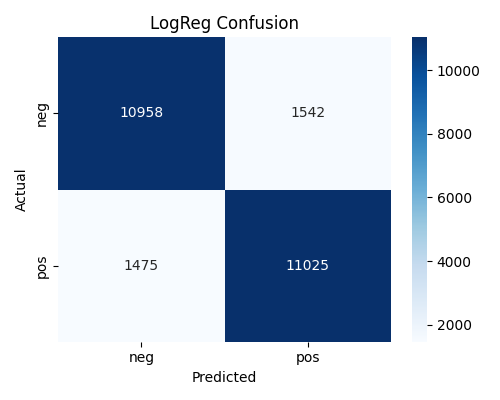
\includegraphics[width=0.6\textwidth]{figures/LogReg_confusion.png}
  \caption{Logistic Regression confusion matrix: TN=10958, FP=1542, FN=1475, TP=11025.}
  \label{fig:confusion_matrix_logreg}
\end{figure}

\begin{figure}[H]
  \centering
  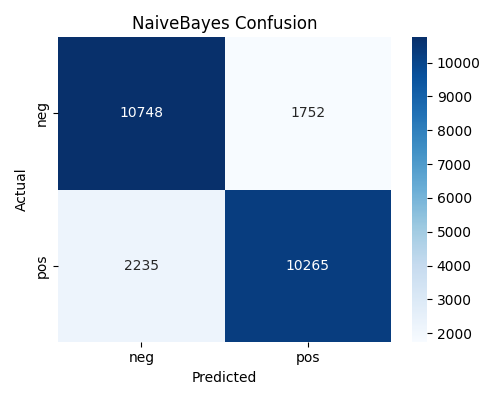
\includegraphics[width=0.45\textwidth]{figures/NaiveBayes_confusion.png}
  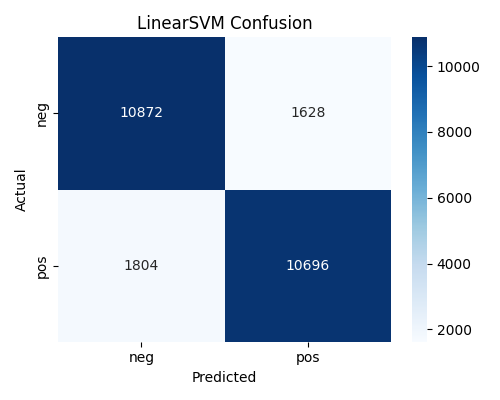
\includegraphics[width=0.45\textwidth]{figures/LinearSVM_confusion.png}
  \caption{Confusion matrices for Multinomial Naïve Bayes (left) and Linear SVM (right).}
  \label{fig:confusion_matrix_nb_svm}
\end{figure}

\subsection{Deep Learning}

\begin{table}[H]
  \centering
  \caption{Test Accuracy after 5 epochs (embed\_dim=100)}
  \label{tab:dl-results}
  \begin{tabular}{lcc}
    \toprule
    \textbf{Model} & \textbf{Test Accuracy} & \textbf{Notes} \\
    \midrule
    LSTM   & 0.511 & Final hidden‐state classifier; underperforms \\
    CNN    & 0.856 & Global max‐pooled conv features \\
    \bottomrule
  \end{tabular}
\end{table}

\noindent
Both models were trained on batches of 64, padded to length 200, using Adam (lr=1e-3). No pretrained embeddings were used. LSTM underperformed significantly, due to insufficient learning.

\begin{figure}[H]
  \centering
  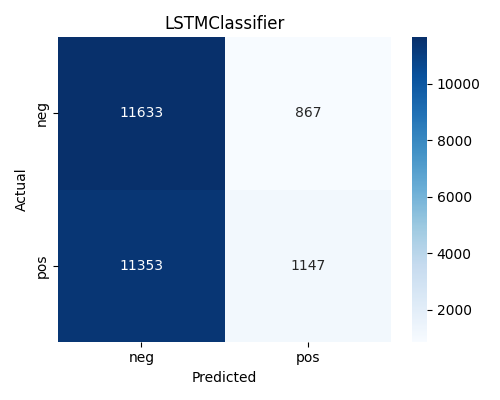
\includegraphics[width=0.45\textwidth]{figures/LSTMClassifier_confusion.png}
  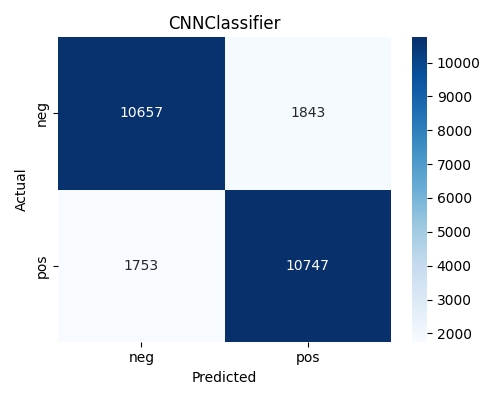
\includegraphics[width=0.45\textwidth]{figures/CNNClassifier_confusion.png}
  \caption{Confusion matrices for LSTM (left) and CNN (right).}
  \label{fig:confusion_matrix_lstm_cnn}
\end{figure}

\section{Discussion}
\begin{itemize}
  \item \textbf{Classical vs.\ Deep:}  
    \begin{itemize}
      \item TF–IDF and Logistic Regression is extremely fast at inference (0.47 ms/sample) with 0.88 accuracy.
      \item CNN improves over classical (0.856 acc), but LSTM underperforms (0.511 acc).
    \end{itemize}
  \item \textbf{Error Analysis:}  
    \begin{itemize}
      \item Classical models struggle with negation (“not good”) and sarcasm.
      \item LSTM has a problem with vanishing gradients and poor convergence.
      \item Short reviews (< 20 words) are most error‐prone across all models.
    \end{itemize}
  \item \textbf{Practical trade‐offs:}  
    \begin{itemize}
      \item For real‐time scoring, Logistic Regression or CNN is better.
    \end{itemize}
\end{itemize}

\section{Conclusion}
We implemented a single‐script pipeline that runs classical and deep methods end‐to‐end on the IMDb dataset. While TF–IDF and Logistic Regression remains a strong, fast baseline (0.88 acc) and CNNs improve slightly (0.856). The LSTM model, despite theoretical potential, failed to train effectively.

\end{document}